\documentclass[12pt,letterpaper]{article}

\usepackage{amsmath} % do komendy \text
\usepackage[margin=0.8in]{geometry}
\usepackage[english]{babel}
\usepackage[utf8]{inputenc}
\usepackage{hyperref}
\usepackage{indentfirst}
\usepackage{graphicx}
\usepackage{fontenc}
\usepackage{caption}
\usepackage{subcaption}
\usepackage{array}
\usepackage{cleveref}
\usepackage{float}
\usepackage{mhchem}
\usepackage{multirow}
\usepackage{stackengine}
\usepackage[backend=biber,style=numeric, sorting=none]{biblatex}

%for showing python code:
\usepackage{listings}
\usepackage{xcolor}
\lstset{
    language=Python, % Set programming language
    basicstyle=\ttfamily\small, % Style of the code font
    keywordstyle=\color{blue}, % Color for keywords
    stringstyle=\color{green!60!black}, % Color for strings
    commentstyle=\color{red}, % Color for comments
    numbers=left, % Line numbers (can be none, left, or right)
    numberstyle=\tiny\color{gray}, % Style for line numbers
    stepnumber=1, % Step between two line numbers
    frame=single, % Adds a frame around the code
    tabsize=4, % Sets tab space
    breaklines=true, % Automatic line breaking
    breakatwhitespace=true, % Break only at whitespace
    showstringspaces=false, % Don't display spaces in strings
}

\addbibresource{references.bib} 

\newlength{\bibparskip}\setlength{\bibparskip}{0pt}
\let\oldthebibliography\thebibliography
\renewcommand\thebibliography[1]{%
  \oldthebibliography{#1}%
  \setlength{\parskip}{\bibitemsep}%
  \setlength{\itemsep}{\bibparskip}%
}
\newcolumntype{M}[1]{>{\centering\arraybackslash}m{#1}}
\newcolumntype{P}[1]{>{\centering\arraybackslash}p{#1}}
\newcommand\xrowht[2][0]{\addstackgap[.5\dimexpr#2\relax]{\vphantom{#1}}}

%my commands
\newcommand{\txt}[1]{\textit{#1}}
\newcommand{\degreeCelsius}{$^\circ$C}
\newcommand{\degree}{$^\circ$}
\newcommand{\nid}{\noindent}
\newcommand{\angstrom}{\mbox{\normalfont\AA}}%do pisania angstremów
\newcommand{\Frac}[2]{\left(\frac{#1}{#2}\right)}
\setlength{\parindent}{3em}

\begin{document}

\begin{center}
    \begin{huge}
     Information distillation from physical simulation\\[12pt]
    \end{huge}
    Damian Gierek\\
    \vspace{0.1em}
    07.02.2025
\end{center}

\hspace{0.3em}

\nid In this paper, I use the method of unsupervised learning of equations of motion for objects in raw and optionally distorted unlabelled synthetic video, presented in this article~\cite{Udrescu2021}, for the case of videos of bodies moving in gravitational field to obtain the trajectories of the bodies. To obtain this, I trained an autoencoder that maps each video frame into a low-dimensional latent space that allows reproducing the original image. The desired 2D Cartesian trajectory is obtained via principal component analysis of vectors from the latent space. The paper presents preliminary results.

\section{Motivation and methodology}

First, let us clarify why this approach is interesting. By obtaining the trajectory of a moving body from a video, we can guess the formula that governs the movement of the body using symbolic regression. An example of an algorithm that allows it is "AI Feynman" \cite{udrescu2020}. This approach was analogous to the work of Johannes Kepler, who discovered that Mars' orbit is an ellipse after analysing the data of its orbit \cite{koyre2013}. 

The method is based on training a specific architecture consisting of an autoencoder and an evolution operator performed on a set of snapshots of a simulation of a body moving in a gravity field.

\section{Code library}
The whole code I used for the project is publicly available here: \url{https://github.com/dgierek/physics_guesser}. 

The library contains the module "data\_generator.py" that is responsible for generating simulation data. The module uses another module called "rocket\_simulation.py" that stores the analytical solutions used in simulation generation. Simulations are stored in the file "simulation\_frames".

The module called "autoencoder.py" contains an implementation of used neural network architecture. Whilst the module "datasets.py" contains data loaders that inherit from torch.utilis.da-\\ta.Dataset and load the simulation data during training sessions. The training loop is implemented in the module called "trainer.py".

Finally, in the "evaluator.py" module I implemented the method for calculating the loss function. The "evaluation.py" module stores the implementation of principal component analysis and visualisation of images and trajectories reconstructed by the neural network.  

\subsection{Simulation of a body moving in a gravity field}

The first problem to solve for the project was to create a set of data with which the neural network will be trained. In the beginning I decided to try to simulate the movement in a gravity or magnetic field, due to harmonic oscillator force and the movement of a free body using numerical integration of differential equations of motion via the Verlet method. Then, I realised it is not necessary as using the analytical solutions is sufficient. Below I show the equations of motion for each type, the analytical solutions I used for simulation and an example of a generated trajectory:

\begin{itemize}
    \item gravity:
    \begin{flushleft}
        \begin{align*}
            \vec{F_g} & = m\vec{g}\\
            x(t) & = \frac{g_x\cdot t^2}{2} + V_{0,x} t + x_0\\
            y(t) & = \frac{g_y\cdot t^2}{2} + V_{0,y} t + y_0,
        \end{align*}
    \end{flushleft}
    \nid where $\vec{F_g}$ is the force of gravity, $m$ is mass of the body (in every calculation $m=1$ was assumed), $\vec{g}$ is the gravity acceleration vector and its $x$ and $y$ components: $g_x$, $g_y$, while $x(t)$, $y(t)$ is the $x$ and $y$ component of the position of the body at a given time $t$. $x_0$ and $y_0$ describe the initial position. $V_{0,x}$ and $V_{0,y}$ describe the initial velocity. An example trajectory was shown on the figure~\ref{fig:exmp_traj_grav}.

    \item magnetic field:
    \begin{flushleft}
        \begin{align*}
            m \ddot{x} & = q \cdot \dot{y} \cdot B_z\\
            m \ddot{y} & = -q \cdot \dot{x} \cdot B_z\\
            x(t) & = x_0 + \frac{1}{\omega}(v_{0,x} \sin{(\omega t)} + v_{0,y} (1 - \cos{(\omega t)}))\\
            y(t) & = y_0 + \frac{1}{\omega}(v_{0,x} (\cos{(\omega t)} - 1) + v_{0,y} \sin{(\omega t)}),
        \end{align*}
    \end{flushleft}
    \nid where double dots represent the second time derivative and single dot represent the first time derivative. $q$ is the electric charge of a body, $B_z$ is the $z$ component of the magnetic field vector (in the 2D case only this component influences the movement) and $\omega=\frac{qB_z}{m}$. An example trajectory was shown on the figure~\ref{fig:exmp_traj_magn}.

    \item harmonic oscillator:
    \begin{flushleft}
        \begin{align*}
            m \ddot{x} & = - k_x (x-r_{0,x})\\
            m \ddot{y} & = - k_y (x-r_{0,y})\\
            x(t) & = (x_0 - r_{0,x}) \cos({\omega_x t}) + \frac{v_{0,x}}{\omega_x} \sin{(\omega_x t)} + r_{0,x}\\
            y(t) & = (y_0 - r_{0,y}) \cos{(\omega_y t)} + \frac{v_{0,y}}{\omega_y} \sin{(\omega_y t)} + r_{0,y},
        \end{align*}
    \end{flushleft}
    \nid where $k_x$, $k_y$ are spring constants in directions $x$ and $y$, $r_{0,x}$ and $r_{0,y}$ are the coordinates of the equilibrium position of the harmonic oscillator (at this point the force acting on the body is $\vec{0}$). $\omega_x=\sqrt{\frac{k_x}{m}}$ and $\omega_y=\sqrt{\frac{k_y}{m}}$. An example trajectory was shown on the figure~\ref{fig:exmp_traj_harm}.

    \item free body movement:
     \begin{flushleft}
        \begin{align*}
            \vec{F_f} & = \vec{0}\\
            x(t) & = x_0 + v_{0,x}t\\
            y(t) & = y_0 + v_{0,y}t.
        \end{align*}
    \end{flushleft}
    \nid An example trajectory was shown on the figure~\ref{fig:exmp_traj_free}.

\begin{figure}[H]
    \centering

        \begin{minipage}{0.49\textwidth}
        
        \centering
        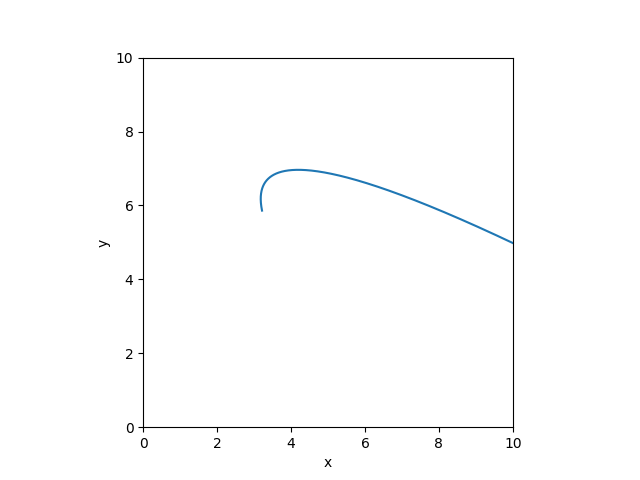
\includegraphics[width=1\linewidth]{example_trajectory_gravity.png}
        \caption{Example trajectory of a body moving in a gravity field. Parameters: $x_{0} = \text{3,22}$, $y_{0} =~\text{5,86}$, $V_{0,x} = -\text{0,17}$, $V_{0,y} = \text{0,82}$, $g_{x} = \text{0,40}$, $g_{y} = -\text{0,31}$.}
        \label{fig:exmp_traj_grav}
        
        \end{minipage}
    \hfill
        \begin{minipage}{0.49\textwidth}
        
        \centering
        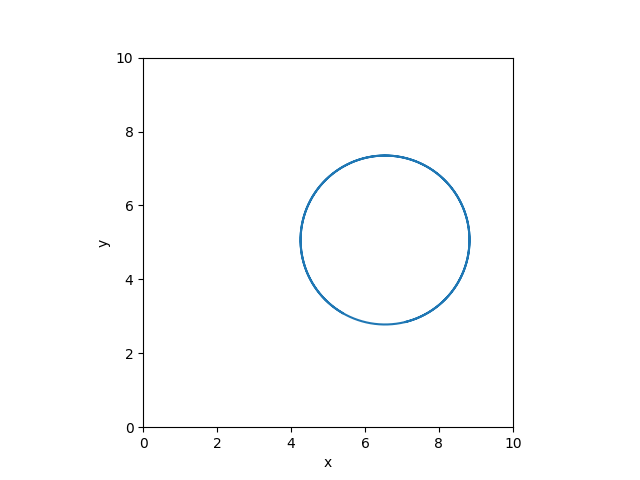
\includegraphics[width=1\linewidth]{example_trajectory_magnetic_field.png}
        \caption{Example trajectory of a body moving in a magnetic field. Parameters: $x_{0} = \text{5,40}$, $y_{0} =~\text{3,09}$, $V_{0,x} = -\text{0,78}$, $V_{0,y} = \text{0,45}$, $B_{z} = \text{0,39}$, $q=1$.}
        \label{fig:exmp_traj_magn}
    
        \end{minipage}    
    
    \end{figure}

    \begin{figure}[H]
        \begin{minipage}{0.49\textwidth}
        
        \centering
        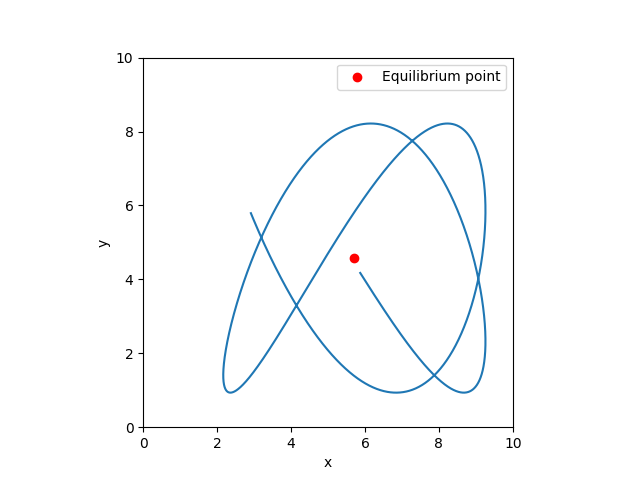
\includegraphics[width=1\linewidth]{example_trajectory_harmonic_oscillator.png}
        \caption{Example trajectory of a body moving due to harmonic oscillator force. The equilibrium position of the harmonic oscillator was also shown. Parameters: $x_{0} = \text{5,87}$, $y_{0} = \text{4,17}$, $V_{0,x} = \text{0,61}$, $V_{0,y} = \text{-0,96}$, $r_{0,x} = \text{5,71}$, $r_{0,y} = \text{4,58}$, $k_{x} = \text{0,03}$, $k_{y} = \text{0,07}$.}
        \label{fig:exmp_traj_harm}
        
        \end{minipage}
    \hfill
        \begin{minipage}{0.49\textwidth}
        
        \centering
        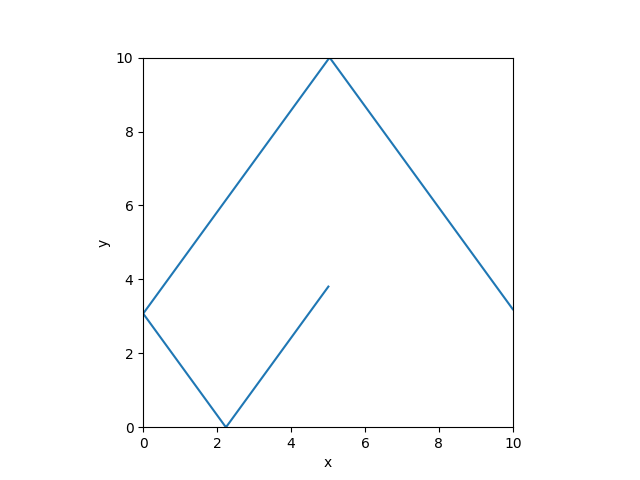
\includegraphics[width=1\linewidth]{example_trajectory_free_body_movement.png}
        \caption{Example trajectory of a body moving freely (no force applied). In this case perfect elastic collisions of the body with walls were implemented. Parameters: $x_{0} = \text{5,01}$, $y_{0} = \text{3,80}$, $V_{0,x} = \text{-0,56}$, $V_{0,y} = \text{-0,77}$.}
        \label{fig:exmp_traj_free}
        
        \end{minipage}  
    \end{figure}
\end{itemize}


For the preliminary results, I used only gravitational simulations. I created 145 simulations with random starting positions, velocities, and directions of the gravity acceleration vector. Each simulation contained about 30 snapshots/frames. Such an example frame is shown in figure~\ref{fig:example_snapshot}.


\begin{figure}[H]

    \centering
    
\includegraphics[width=0.3\textwidth]{example_snapshot.png}
    \caption{An example snapshot of one of the simulations of a body (the red rectangle) moving in a gravity field on the blue background.}
    \label{fig:example_snapshot}

\end{figure}

\subsection{Neural network architecture}

The neural network architecture consists of autoencoder (encoder and decoder) and an evolution operator. The encoder consists of five convolutional ReLU layers (torch.nn.Conv2d and torch.nn.ReLU from PyTorch library) with kernel size 4 and padding 1, four of them with stride 2 followed by one with stride 1. At the end there is a fully connected linear layer (torch.nn.Linear) that gives a latent space vector of dimension 10. The number of channels goes from 3 for the input image to 32, 32, 64, 64 and 256 for the convolutional layers. The decoder network is a mirror image of the encoder in terms of layer dimensions, with the convolution layers replaced by deconvolution layers (torch.nn.ConvTranspose2d). The evolution operator has three fully connected 32-neuron layers (torch.nn.Linear) with softplus activation function (torch.nn.Softplus) and a linear 10-neuron output layer. The evolution operator takes two vectors from latent space (the vector from the current and the previous time step) and predicts the latent space vector for the next time step.
A graphical illustration of the architecture is shown in figure~\ref{fig:neural_net_architecture}.

\begin{figure}[H]
    \centering
    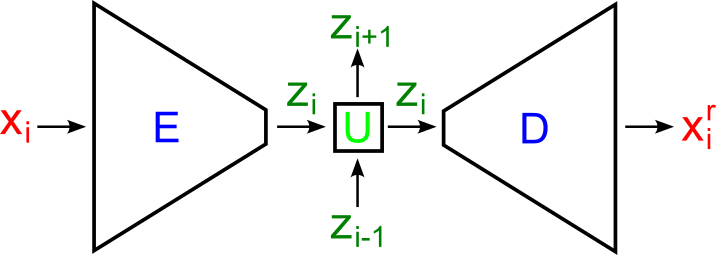
\includegraphics[width=0.5\linewidth]{architecture.png}
    \caption{A draft of a neural network architecture consisting of encoder - E, decoder - D and an evolution operator - U. Encoder E encodes a snapshot from a video (a frame of a video with the moving body) - $x_i$ into a low dimensional latent space vector $z_i$. The evolution operator U takes the latent space vector $z_i$ and the latent space vector from a previous simulation time step - $z_{i-1}$ (we receive it by encoding $x_{i-1}$), and returns the prediction of latent space vector of the following time step $z_{i+1}$. Then, the decoder D decodes the latent space vector $z_i$ and returns the reconstructed snapshot from the video - $x_i^r$. In subsection~\ref{subs:implement_train_loop} an implementation of the training loop of the network was presented. The symbols used on the figure correspond to the variables used in the code, in the following way: $x_i=\text{x\_curr}$, $z_i=\text{z\_curr}$, $z_{i-1}=\text{z\_prev}$, $z_{i+1}=\text{z\_next\_pred}$, $x_i^r=\text{reconstructed}$ (in the code these variables appear for example in the line 57).}
    \label{fig:neural_net_architecture}
\end{figure}

\subsection{Loss function}
\label{subs:loss_function}

The loss function~\cite{Udrescu2021} was implemented as follows:

\begin{equation*}
    \mathcal{L} = \mathcal{L}^{recon} + \alpha\mathcal{L}^{pred} + \beta\mathcal{L}^{nl} + \gamma\mathcal{L}^{acc}. 
\end{equation*}

\nid These four terms are averages over all time steps \txt{i} of the following functions:

\begin{flushleft}
    \begin{align*}
        \mathcal{L}^{recon}_i & = \frac{|x_i-D(E(x_i))|}{|x_i|},\\
        \mathcal{L}^{pred}_i & = \frac{|z_{i+1} - U(z_i, z_{i-1})|}{|z_i - z_{i-1}|},\\
        \mathcal{L}^{nl}_i & = \frac{1}{4000}|z_i - z_{i-1}|\cdot||\nabla\boldsymbol{J}(\boldsymbol{w}_i)||_1,\\ 
        \mathcal{L}^{acc}_i & = \frac{1}{10}||U(\boldsymbol{w}_i) - \boldsymbol{M}\boldsymbol{w}_i||_1,
    \end{align*}
\end{flushleft}

\nid where $\alpha$, $\beta$, $\gamma$ are tunable hyperparameters, $\mathbf{w}_i = \begin{pmatrix} z_{i-1} \\ z_{i} \end{pmatrix}$, $\boldsymbol{J}$ is the Jacobian of an evolution operator U, $\boldsymbol{M} = \begin{pmatrix} -\boldsymbol{I} & 2\boldsymbol{I} \end{pmatrix}$ and $\boldsymbol{I}$ is the 10x10 identity matrix. 

$\mathcal{L}^{recon}$ is the reconstruction error - it simply tells how good the encoder-decoder architecture preserves the input image, which we want to as good as possible. $\mathcal{L}^{pred}$ is the prediction error which tells how well the evolution operator \txt{U} predicts the next latent space vector from two previous ones, which we also want to be as good as possible, so that the dynamics of the moving body is described well. $\mathcal{L}^{nl}$ is a measure of the nonlinearity of the mapping \txt{U}, since its Jacobian $\boldsymbol{J}$ will be constant if the mapping is linear, i.e. the dynamics of the body is described by coupled linear differential equations, which encompass behaviour such as motion in magnetic fields, harmonic oscillator potential and gravity. $\mathcal{L}^{acc}$ is along with $\mathcal{L}^{nl}$ yet another measure of the nonlinearity of the mapping U and is a measure of the predicted acceleration. There is no acceleration if the mapping is $U(\boldsymbol{w}) = \boldsymbol{M}\boldsymbol{w}$.

\subsection{Implementation of the training loop}
\label{subs:implement_train_loop}

In this subsection I presented the code implementation of the training loop. Code comments describe what each chunk of code does. Please take notice on the comment in the line 67, which describes the error made in the implementation of the training loop.   
\begin{lstlisting}
# Importing the necessary functions and classes from third party libraries (like torch) and from scripts I created myself (like autoencoder)
from torch import device, cuda, save
from torch.optim import Adam
from autoencoder import AutoencoderWithEvolution
from datasets import ImageDataset, collate_fn
from torch.utils.data import DataLoader
from torchvision import transforms
from evaluator import CombinedLoss
from tqdm import tqdm
import matplotlib.pyplot as plt

# Using GPU if available
device = device('cuda' if cuda.is_available() else 'cpu')
print('Device:', str(device))

# Initialising our autoencoder:
model = AutoencoderWithEvolution().to(device)

# Defining transformation of images:
transform = transforms.Compose([
    transforms.Resize((64, 64)),  # down sampling the resolution of the images
    transforms.ToTensor()])

# Defining the class for calculating the loss function - criterion and an optimizer for training - optimizer
criterion = CombinedLoss(alpha=1.0, beta=1.0, gamma=1.0)
optimizer = Adam(model.parameters(), lr=1e-3)

num_epochs = 145 # 1 epoch is equivalent to training on one whole simulation (approximately 30 frames)

# Defining tables that will store losses values after each epoch for latter plotting
total_Loss = []
total_reconstruction_Loss = []
total_prediction_error_Loss = []
total_non_linearity_Loss = []
total_acceleration_Loss = []

for epoch in range(num_epochs):

    # Getting data out of one of the gravity simulations:
    dataset = ImageDataset(directory=rf'simulation_frames/gravity_{epoch}/
                                        simulation_snapshots', transform=transform)
    dataloader = DataLoader(dataset, batch_size=1, shuffle=False, collate_fn=collate_fn)

    total_loss = 0
    total_reconstruction_loss, total_prediction_error_loss, total_non_linearity_loss, total_acceleration_loss = (
        0, 0 ,0 ,0)
    for _, data in tqdm(dataloader):
        # Getting snapshots out of one of the gravity simulations:
        x_prev, x_curr, x_next = data.squeeze(0).to(device)
        x_prev = x_prev.unsqueeze(0).requires_grad_(True)
        x_curr = x_curr.unsqueeze(0).requires_grad_(True)
        x_next = x_next.unsqueeze(0).requires_grad_(True)

        optimizer.zero_grad()

        # Encode and decode current frame using our model
        reconstructed, z_curr, z_next_pred = model(x_curr, z_prev=model.encoder(x_prev))

        # Encode next frame to get the ground truth z_next
        z_next_true = model.encoder(x_next)

        # Compute losses
        reconstruction_loss, prediction_error_loss, non_linearity_loss, acceleration_loss, loss = criterion(
            reconstructed, x_curr, x_next, z_prev=model.encoder(x_prev), z_curr=z_curr,
            z_next_pred=z_next_pred, z_next_true=z_next_true, latent_dim=10)

        # Backpropagation and optimization (this is erroneous as we should perform backpropagation after going through all time steps in one simulation - the following lines should be inside the outer loop)
        loss.backward()
        optimizer.step()

        # Summing up losses
        total_loss += loss.item()
        total_reconstruction_loss += reconstruction_loss.item()
        total_prediction_error_loss += prediction_error_loss.item()
        total_non_linearity_loss += non_linearity_loss.item()
        total_acceleration_loss += acceleration_loss.item()

    # Printing losses after each epoch
    print(f"Epoch {epoch + 1}, total loss: {total_loss / len(dataloader):.4f}")
    print(f"Epoch {epoch + 1}, reconstruction loss: {total_reconstruction_loss / len(dataloader):.4f}")
    print(f"Epoch {epoch + 1}, prediction error loss: {total_prediction_error_loss / len(dataloader):.4f}")
    print(f"Epoch {epoch + 1}, non linearity loss: {total_non_linearity_loss / len(dataloader):.4f}")
    print(f"Epoch {epoch + 1}, acceleration loss: {total_acceleration_loss / len(dataloader):.4f}")

    # Saving the calculated losses for latter plotting
    total_Loss.append(total_loss / len(dataloader))
    total_reconstruction_Loss.append(total_reconstruction_loss / len(dataloader))
    total_prediction_error_Loss.append(total_prediction_error_loss / len(dataloader))
    total_non_linearity_Loss.append(total_non_linearity_loss / len(dataloader))
    total_acceleration_Loss.append(total_acceleration_loss / len(dataloader))

# Saving the model
save(model.state_dict(), r'saved_models/trained_on_10_simulations.pth')
\end{lstlisting}

\section{Preliminary results}

After performing a training session on all the simulations of a body moving in a gravity field I realised a big flaw in my training loop. Namely, the loss function was not calculated as described in subsection~\ref{subs:loss_function} as an average of all time steps in one simulation but after each frame. For in code details, see~\ref{subs:implement_train_loop}. Although the components of the loss function appeared to get smaller during training session, after visualizing the reconstructed images of snapshots of a simulation and comparing them with original images, it is clear that something is wrong. The graph of the values of loss function and its components with respect to the training epoch is presented in figure~\ref{graph:loss_function_vs_epoch_number}. The comparison between an original image and the reconstructed one is shown in figure~\ref{fig:original_reconstructed_image}. 

I have also created an image of a reconstructed trajectory. By comparing it with the original trajectory, one could think it seems to be almost correct (neglecting some rotations and linear scaling). However, in my opinion, since I used flawed training loop, it is rather a coincidence. The comparison between an original trajectory with the reconstructed one is shown in figure~\ref{fig:original_reconstructed_trajectory}.

\begin{figure}[H]
    \centering
    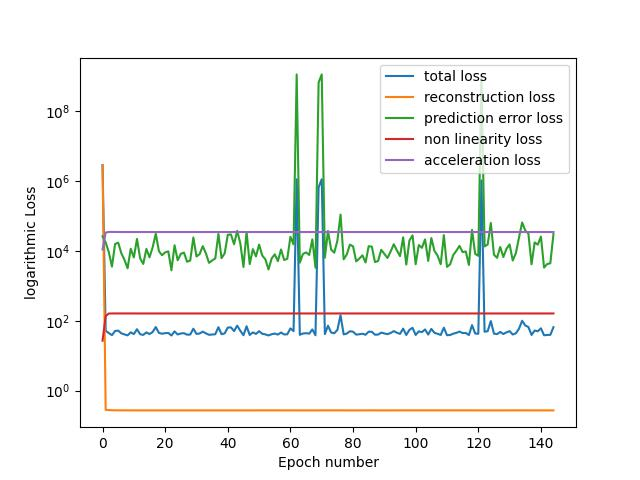
\includegraphics[width=0.5\linewidth]{trained_on_145_simulations_loss.jpg}
    \caption{Components of the loss function versus epoch number during training. Each epoch corresponds to training performed on one simulation.}
    \label{graph:loss_function_vs_epoch_number}
\end{figure}

\begin{figure}[H]
    \centering

    \begin{minipage}{0.49\textwidth}
    
    \centering
    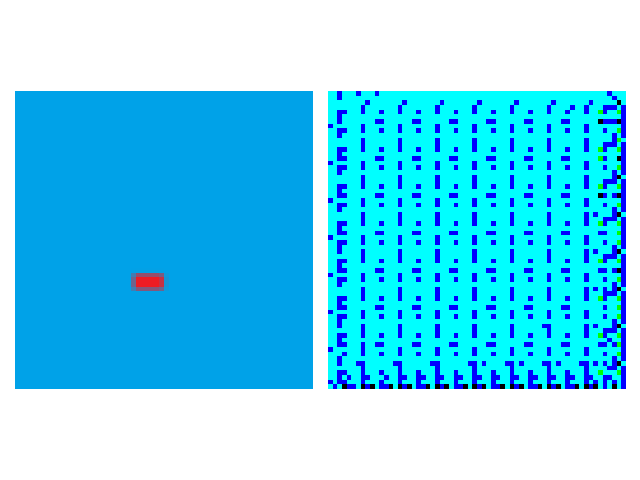
\includegraphics[width=1\textwidth]{original_image_and_reconstructed_image.png}
    \caption{The comparison between original snapshot of a simulation (the photo is blurred as the images entering encoder are deliberately downsampled) on the left and the reconstructed image on the right. It is clear that reconstruction went wrong.}
    \label{fig:original_reconstructed_image}
    
    \end{minipage}
    \hfill
    \begin{minipage}{0.49\textwidth}
    
    \centering
    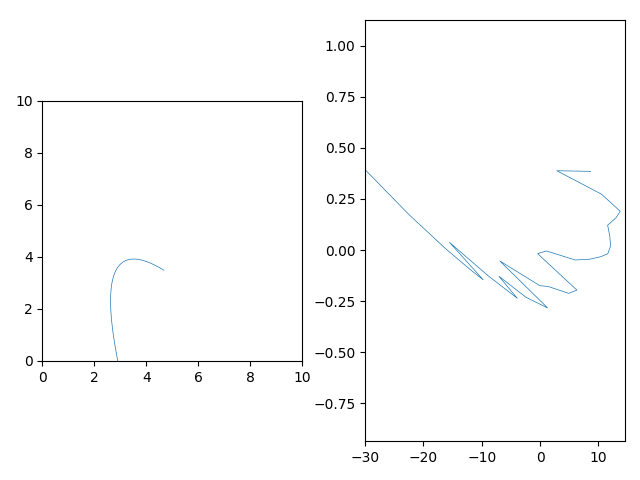
\includegraphics[width=1\textwidth]{original_trajectory_and_reconstructed_one.png}
    \caption{The comparison between an original trajectory of a body on the left with the reconstructed trajectory on the left.}
    \label{fig:original_reconstructed_trajectory}

    \end{minipage}    
    
\end{figure}


\section{Summary and future work}

In the paper I presented the preliminary results of my attempt to reproduce the results of the article~\cite{Udrescu2021}. For now, I did not manage to obtain a correctly working algorithm that reconstructs the trajectory of a moving object from a video due to a flawed training loop procedure.

In the future work, I will concentrate on repairing the issue with training loop and try to obtain the desired results. The work that is still ahead is implementing a comprehensive evaluator that would assess the quality of latent space trajectory representations and extending the training of the model on other types of motion like movement in magnetic field, harmonic oscillator. In the end it would be interesting to see, if the neural network architecture would be able to detect the trajectories of bodies from real footages.  

\printbibliography

\end{document}
